\textbf{Computing Integral Image}

I have computed integral image using the following algorithm

\[
II[i, j] = I[i, j] + II[i-1, j] + II[i, j-1] - II[i-1, j-1]
\]

where I is the original image and II is the integral image.

\textbf{Haar-like features}

I have used the four type of Haar-like features as shown in the figure below.

\begin{figure}[H]
    \centering
    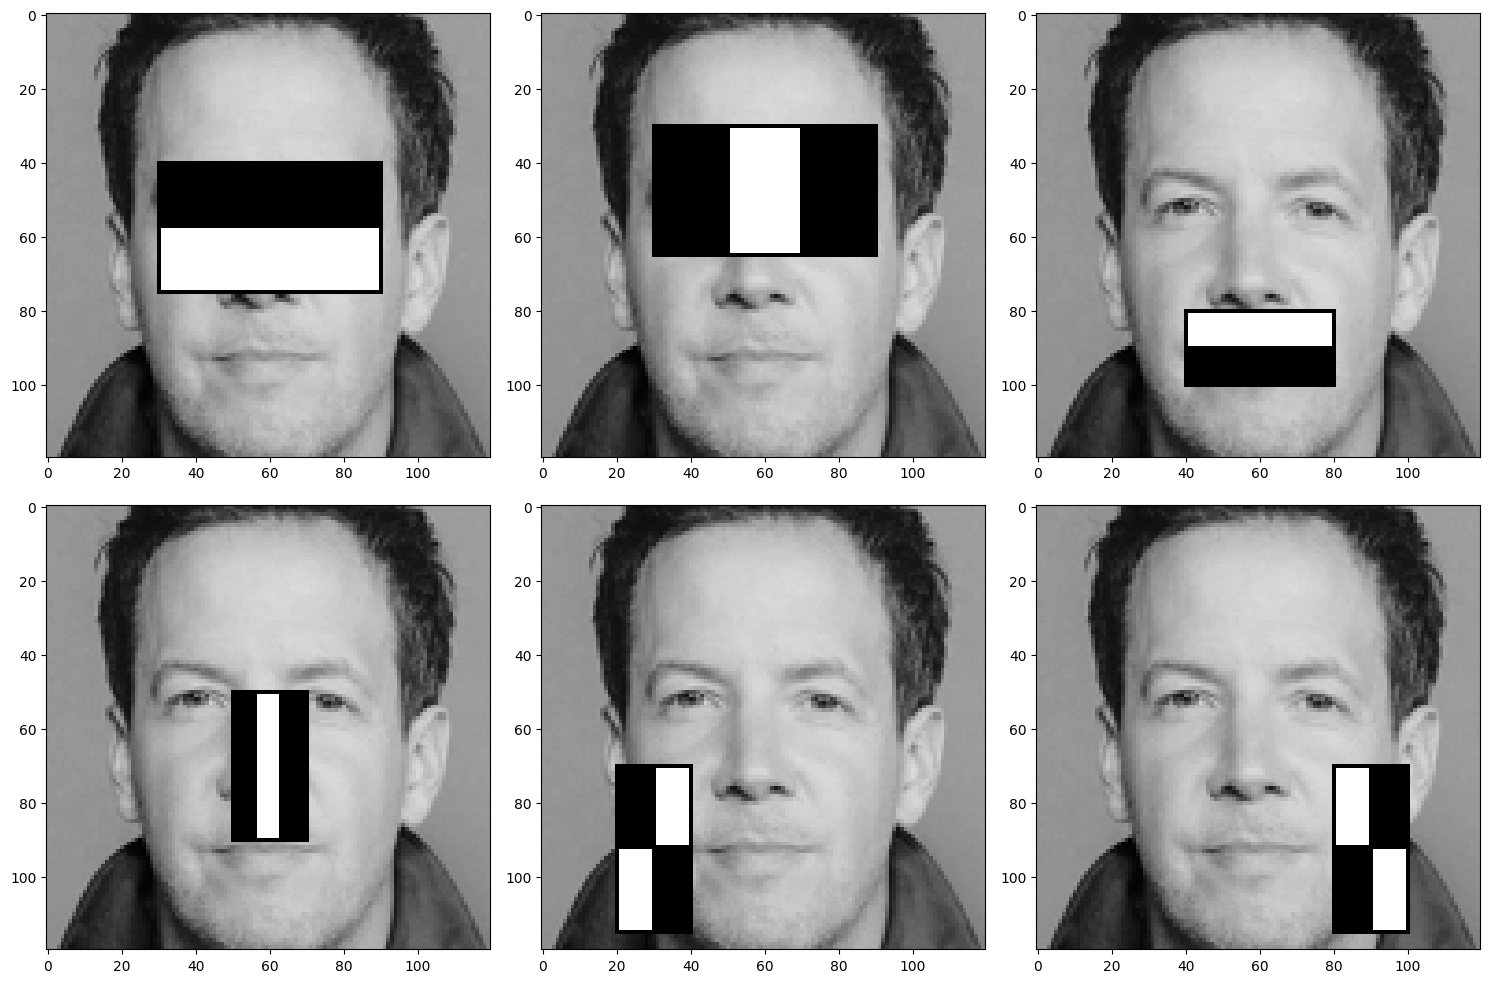
\includegraphics[width=.7\textwidth]{imgs/haar_like_features.png}
    \caption{Haar-like features}
    \label{fig:2_mediapipe}
\end{figure}

\textbf{Face Detection}

I have seletected first, second and fourth Haar-like features to detect face. I have used the following algorithm to detect face.

\begin{itemize}
    \item Check if the first haar-like feature evaluate to $>1.8$
    \item Check if the second haar-like feature evaluate to $>.8$
    \item Check if the fourth haar-like feature evaluate to $>.35$
\end{itemize}

If all the above conditions are satisfied then the face is detected, else the blcok is rejected.

\textbf{Results}

Applied my face detection algorithm on image with faces and the results were as follows.

\begin{figure}[H]
    \centering
    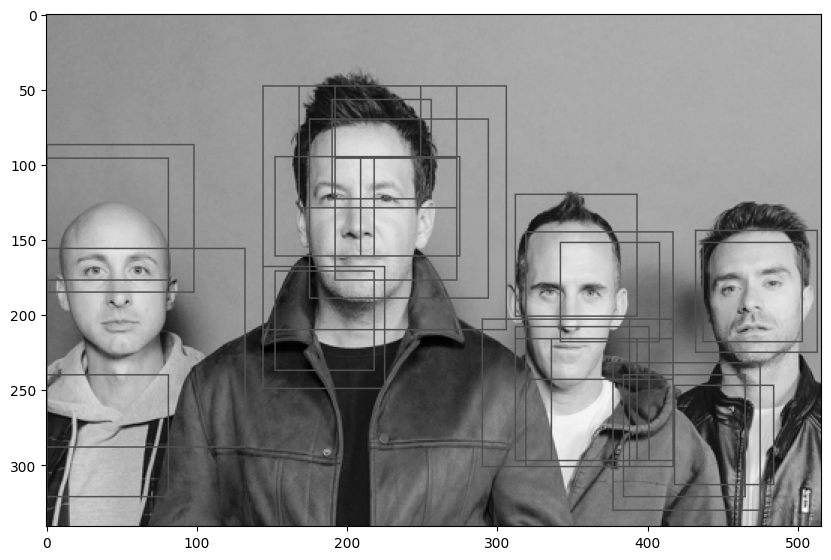
\includegraphics[width=.9\textwidth]{imgs/face_detected.png}
    \caption{Face detection performance}
    \label{fig:2_mediapipe}
\end{figure}


Though all the four faces are detected, the face detection algorithm is not very accurate. There are too many false positives. This is because I have consider only three features which is not enough to describe the face.

\newpage